\documentclass[12pt,x11names,a4paper]{article}
%Preamble

\usepackage{comment}
\usepackage[utf8]{inputenc}
\usepackage{amsmath}
\usepackage{amssymb}
\usepackage{amsthm}
\usepackage{enumitem}
\usepackage{mathrsfs}
\usepackage{mathtools}
\usepackage{esvect}
\usepackage{xfp}
\usepackage{xparse}
\usepackage{array}
\usepackage{changepage}
\usepackage{pdfpages}
\usepackage[parfill]{parskip}
\usepackage{anyfontsize}
\usepackage{alphalph}
\usepackage{ulem}
\usepackage{cancel}
\usepackage[framemethod=tikz]{mdframed}
\usepackage{xargs}
\usepackage{siunitx}              


\usepackage{algorithm}
\usepackage{algorithmic}
\usepackage{matlab-prettifier}
\usepackage{textcomp}
\usepackage{listings}
\usepackage[dvipsnames,svgnames]{xcolor}
\usepackage{colortbl}
\usepackage{eso-pic}
\usepackage[a4paper, margin=24mm]{geometry}
\usepackage{float}
\usepackage[danish]{babel}
\usepackage{tikz}
\usetikzlibrary{matrix,calc}
\usetikzlibrary{arrows}
\usetikzlibrary{arrows.meta}
\usetikzlibrary{decorations.pathreplacing}
\usetikzlibrary{decorations.pathreplacing,calligraphy}
\usetikzlibrary{patterns}
\usetikzlibrary{angles, quotes}
\usepackage{csquotes}
\usepackage{pdfpages}
\usepackage{fancyhdr}
\usepackage{lastpage}
\usepackage{pgfplots}
\usepackage{pgffor}

%Ændre følgende, hvis du vil have en anden bredde på pgfplots
\pgfplotsset{width=10cm,compat = 1.9}




\usepackage{caption}
\usepackage{subcaption}
\makeatletter
% \def\@seccntformat#1{%
%   \expandafter\ifx\csname c@#1\endcsname\c@section\else
%   \csname the#1\endcsname\quad
%   \fi}
 \makeatother
\counterwithin*{equation}{section}
\numberwithin{equation}{section}



%\newtheorem{setn}{Sætning}[section]
%\newtheorem{prop}[defn]{Proposition}
%\newtheorem{lem}[defn]{Lemma}
%\newtheorem{cor}[defn]{Korollar}

\newcommand\Tr{\textnormal{Tr}}
\newcommand\N{\textnormal{N}}
\newcommand{\suco}[2]{\left.#1\right|_{\mathbb{F}_{#2}}}
\renewcommand\qedsymbol{$\blacksquare$}
\theoremstyle{definition}
%\newtheorem{defn}[setn]{Definition}

\newcommand\Ker{\textnormal{Ker}\hspace{0.5mm}}
\renewcommand\Im{\textnormal{Im}\hspace{0.5mm}}
\newcommand\TS{\hspace{0.8mm}}

\usepackage{tcolorbox}
\tcbuselibrary{theorems}

\newmdtheoremenv[
	skipabove = 5pt,
	skipbelow = 5pt,
	roundcorner = 5,
	backgroundcolor = SeaGreen!30,
	linecolor = white, 
	]
	{defn}{Definition}[section]

\newmdtheoremenv[
	skipabove = 5pt,
	skipbelow = 5pt,
	roundcorner = 5,
	backgroundcolor = Melon!25,
	linecolor = white, 
	]
	{setn}[defn]{Sætning}
	
\newmdtheoremenv[
	skipabove = 5pt,
	skipbelow = 5pt,
	roundcorner = 5,
	backgroundcolor = Melon!25,
	linecolor = white, 
	]
	{lem}[defn]{Lemma}

\newtheorem{eksempel}[defn]{Eksempel}

\newenvironment{exa}
	{\begin{eksempel}}
	{\unskip\hfill $\square$ \end{eksempel}}
\newtheorem{regel}[defn]{Regel}


\usepackage{graphicx}
\usepackage[backend=biber]{biblatex}
\addbibresource{biblio.bib}

\renewcommand{\mod}[1]{\ (\textnormal{mod }{#1})}
\newcommand{\fmod}[1]{\ \textbf{mod }{#1}}
\usepackage{hyperref, bookmark}
\usepackage{booktabs}
\usepackage{calc}
\usepackage[nottoc,numbib]{tocbibind} 
\usepackage{multirow,bigdelim}

\renewcommand{\arraystretch}{1.3}
\newcommand\intd{\textnormal{d}}
\newcommand\e{\textnormal{e}}




\newenvironment{opgavetekst}[1]
{
	\begin{minipage}[t]{0.15\textwidth}
	 	\textbf{ #1}
	\end{minipage}
	\begin{minipage}[t]{0.85\textwidth}
		\rule{\textwidth}{0.3mm} \\
}
{ 
\\	\end{minipage}
}

\newenvironment{meretekst}
{
	\begin{minipage}[t]{0.15\textwidth}
	 	\phantom{h}
	\end{minipage}
	\begin{minipage}[t]{0.85\textwidth}
}
{ 
\\	\end{minipage}
}

\newenvironment{delopgave}[1]
{
	\begin{minipage}[t]{0.15\textwidth}
		\phantom{\textbf{Opgave}}		
		\textbf{\symbol{\numexpr96+ #1})}
	\end{minipage}
	\begin{minipage}[t]{0.85\textwidth}

	\begin{minipage}[t]{\textwidth}
}{
\end{minipage}
\phantom{h}\\
\end{minipage}
}

\newcommand{\cis}{\textnormal{\hspace{0.5mm}cis}}
%\newcommand{opgavelinje}[1]{
%\begin{minipage}[t]{0.15\textwidth}
%\textbf{#1}
%\end{minipage} 
%\begin{minipage}[t]{\textwidth}
%\rule{0.81\textwidth}{0.3mm}
%\end{minipage}
%}





%Farver!
\definecolor{NorregGroen}{RGB}{0,105,78}





\newgeometry{margin=2cm}

\pagestyle{fancy}
\fancyhf{}

\rhead{Nørre Gymnasium\\3.e	
}
\cfoot{Side \thepage \hspace{1pt} af \pageref{LastPage}}

%Husk at rette modul og dato!
\lhead{Aflevering 1\\ Matematik A }%<---------------------------------------RET
\chead{28. august 2026}%<----------------------------------------------------RET


\begin{document}

%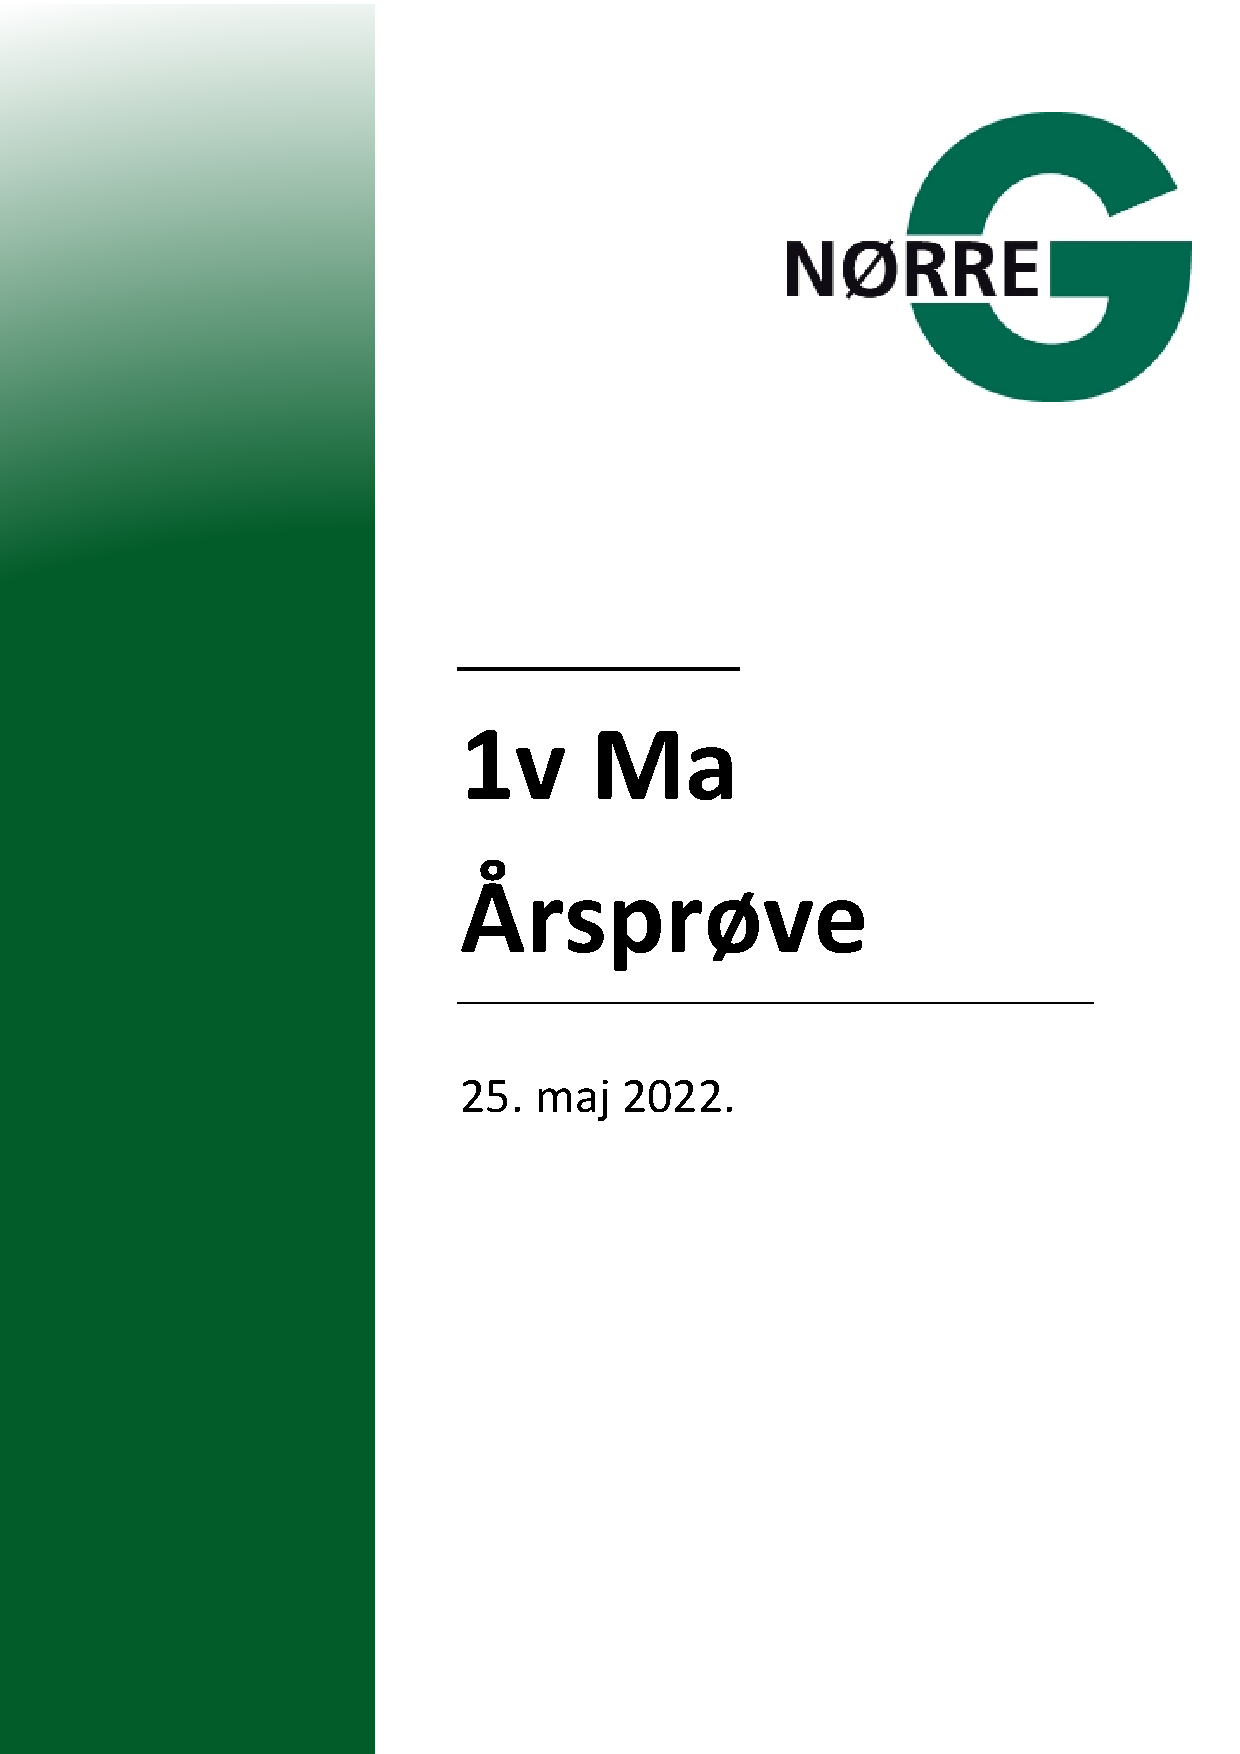
\includepdf[pages=-]{Forsider/aarsprove_1v.pdf}
\savegeometry{art}

\begin{titlepage}
\newgeometry{margin=0pt}

\begin{minipage}{0.27\textwidth}

\begin{tikzpicture}[overlay]
\fill[top color = NorregGroen!40, bottom color = NorregGroen] (6,10) rectangle (-10,-30);
\end{tikzpicture}
\end{minipage}
\begin{minipage}{0.73\textwidth}
\begin{center}
\phantom{h} \vspace{1cm}\\
\hspace{4cm}

\includegraphics[scale = 1]{Billeder/Norreg.png} \\
\phantom{h} \vspace{5cm}\\
\rule{0.7\textwidth}{0.3mm}\\
\phantom{h}\\
{\fontsize{50}{60}\selectfont Aflevering 1}\\%<---------------------------------------RET
\phantom{h}\\
\rule{0.7\textwidth}{0.3mm}\\
\Large 2026\\
\Large 3.e MA

\end{center}
\end{minipage}
\end{titlepage}
\loadgeometry{art}

%Udfyld afsnit herunder og lav til egen Latex-fil

%Kopier følgende til overskrift:

%\begin{center}
%\Huge
%Aflevering 1
%\end{center}
%\section*{Opgave 1}
%\stepcounter{section}
\begin{center}
%Opgavesætter er delt i to dele:\\
%Delprøve 1 kun med den centralt udmeldte formelsamling.\\
%Delprøve 2 med alle hjælpemidler.
\end{center}

\section*{Krav til formidling af din besvarelse}

Ved bedømmelse af helhedsindtrykket af besvarelsen af de enkelte opgaver lægges særlig vægt på følgende fire punkter:
\begin{itemize}
\item[$\cdot$] \textbf{Redegørelse og dokumentation for metode} \\
Besvarelsen skal indeholde en redegørelse for den anvendte løsningsstragegi med dokumentation i form af et passende antal mellemregninger \textit{eller} matematiske forklaringer på metoden, når et matematisk værktøjsprogram anvendes.
\item[$\cdot$] \textbf{Figurer, grafer og andre illustrationer} \\
Besvarelsen skal indeholde hensigtsmæssig brug af figurer, grafer og andre illustrationer, og der skal være tydelige henvisninger til brug af disse i den forklarende tekst.
\item[$\cdot$] \textbf{Notation og layout}\\
Besvarelsen skal i overensstemmelse med god matematisk skik opstilles med hensigtsmæssig brug af symbolsprog, og med en redegørelse for den matematiske notation, der indføres og anvendes, og som ikke kan henføres stil standardviden.
\item[$\cdot$] \textbf{Formidling og forklaring}\\
Besvarelsen af rene matematikopgaver skal indeholde en angivelse af givne oplysninger og korte forklaringer knyttet til den anvendte løsningsstrategi beskrevet med brug af almindelig matematisk notation. 

Besvarelsen af opgaver, der omhandler matematiske modeller, skal indeholde en kort præsentation af modellens kontekst, herunder betydning af modellens parametre. De enkelte delspørgsmål skal afsluttes med en præcis konklusion præsenteret i et klart sprog i relation til konteksten.
\end{itemize}

\newpage
\begin{center}
	\LARGE
	Uden hjælpemidler
\end{center}
\begin{opgavetekst}{Opgave 1}
\end{opgavetekst}
\begin{delopgave}{1}
	Reducer udtrykket $(a + b)(a - b) + b^2 - 2a^2$.
\end{delopgave}
%
%
%
%
%
%
\begin{opgavetekst}{Opgave 2}
\end{opgavetekst}
\begin{delopgave}{1}
	Bestem grænseværdien for følgende $0/0$-udtryk:
	\begin{align*}
		\lim_{x \to 4} \frac{x^2 - 16}{x - 4}.
	\end{align*}
\end{delopgave}
%
%
%
%
%
\begin{opgavetekst}{Opgave 3}
	En funktion $f$ er givet ved 
	\begin{align*}
		f(x) = \ln(x^2).
	\end{align*}
\end{opgavetekst}
\begin{delopgave}{1}
	Bestem $f'(x)$.
\end{delopgave}
\begin{delopgave}{2}
	Bestem ligningen for tangenten til $f$ i punktet $P(1,f(1))$.
\end{delopgave}
%
%
%
%
%
\begin{opgavetekst}{Opgave 4}
	På Figur \ref{fig:arealer} kan vi se grafen for en funktion $f$ samt arealet $A$, der afgrænses af grafen for $f$ og $x$-aksen. Funktionen $f$ har forskriften
	\begin{align*}
		f(x) = x^3 - x^2 - 2x.
	\end{align*}
	\begin{figure}[H]
		\centering
		\begin{tikzpicture}
		\begin{axis}[
		axis lines = middle,
		xmin = -2, xmax = 3,
		ymin = -5, ymax = 5,
		xlabel = {$x$}, ylabel = {$y$},
		xtick = {-2,-1,0,...,3},
		ytick = {-5,-4,...,5},
		grid = both
		]
			\addplot[color = SeaGreen, thick, domain = -2:3, samples = 200] {x^3 - x^2 - 2*x};
			\filldraw[domain = -1:2, color = SeaGreen!40, opacity = 0.4, samples = 200] (axis cs: -1,0) -- plot (axis cs: \x, \x*\x*\x - \x*\x - 2*\x) -- (axis cs: 2,0) -- cycle;
			\node[color = SeaGreen] at (axis cs: 2.5,2.5) {$f$};
			\node[color = SeaGreen] at (axis cs: 2.5,2.5) {$f$};
		\end{axis}
		\end{tikzpicture}
		\caption{Graf for funktionen $f$ med arealet $A$ markeret.}
		\label{fig:arealer}
	\end{figure}
	\phantom{h}
\end{opgavetekst}
\begin{delopgave}{1}
	Vis, at arealet $A = \frac{37}{12}$.
\end{delopgave}
%
%
%
%
%
\begin{opgavetekst}{Opgave 5}
	En trekant $\triangle ABC$ er givet på Figur \ref{fig:trekant}.
	\begin{figure}[H]
		\centering
		\begin{tikzpicture}
			\draw[color = SeaGreen, thick] (0,0) -- (10*0.6,0) node[midway, anchor = north] {$10$} 
			node[pos = 0, anchor = north east] {$A$} node[pos = 1, anchor = north west] {$C$};
			\draw[color = SeaGreen, thick] (0,0) -- (5*0.6,6.25*0.6) node[midway, anchor = south east] {$8$}
			node[pos = 1, anchor = south] {$B$};
			\draw[color = SeaGreen, thick] (5*0.6,6.25*0.6) -- (10*0.6,0) node[midway, anchor = south west] {$8$};
		\end{tikzpicture}
		\caption{Trekanten $\triangle ABC$.}
		\label{fig:trekant}
	\end{figure}
	\phantom{h}
\end{opgavetekst}
\begin{delopgave}{1}
	Vis, at $\cos(\angle A) = \frac{5}{8}$.
\end{delopgave}
%
%
%
%
%
\newpage
\begin{opgavetekst}{Opgave 6}
	To vektorer $\vv{a}$ og $\vv{b}$ er givet ved
	\begin{align*}
		\vv{a} = \begin{pmatrix}
			t \\ -1
		\end{pmatrix}
	\quad \textnormal{og} \quad
		\vv{b} = \begin{pmatrix}
			t-1 \\ 6
		\end{pmatrix}.
	\end{align*}
\end{opgavetekst}
\begin{delopgave}{1}
	Bestem de værdier for $t$, så $\vv{a}$ og $\vv{b}$ er ortogonale.
\end{delopgave}
%
%
%
%%
%
\begin{opgavetekst}{Opgave 7}
	En cirkel $c$ er givet ved ligningen
	\begin{align*}
		c:\  x^2 + y^2 - 4x - 6y + 9 = 0.
	\end{align*}
\end{opgavetekst}
\begin{delopgave}{1}
	Bestem centrum og radius for cirklen $c$.
\end{delopgave}	
%
%
%%%%%%%%%%%%%%%
%
%
\newpage
\begin{center}
	\LARGE
	Med hjælpemidler
\end{center}
%
%
%
\begin{opgavetekst}{Opgave 8}
	To linjer $l$ og $m$ er givet ved henholdsvis
	\begin{align*}
		&l: \ 5x + 19y = 12, \\
		&m: \ 10x -10y = 29.
	\end{align*}
\end{opgavetekst}
\begin{delopgave}{1}
	Bestem skæringspunktet mellem $l$ og $m$.
\end{delopgave}
\begin{delopgave}{2}
	Brug en formel til at bestemme den spidse vinkel mellem $l$ og $m$.
\end{delopgave}
%
%
%
%
%
\begin{opgavetekst}{Opgave 9}
	\begin{center}
		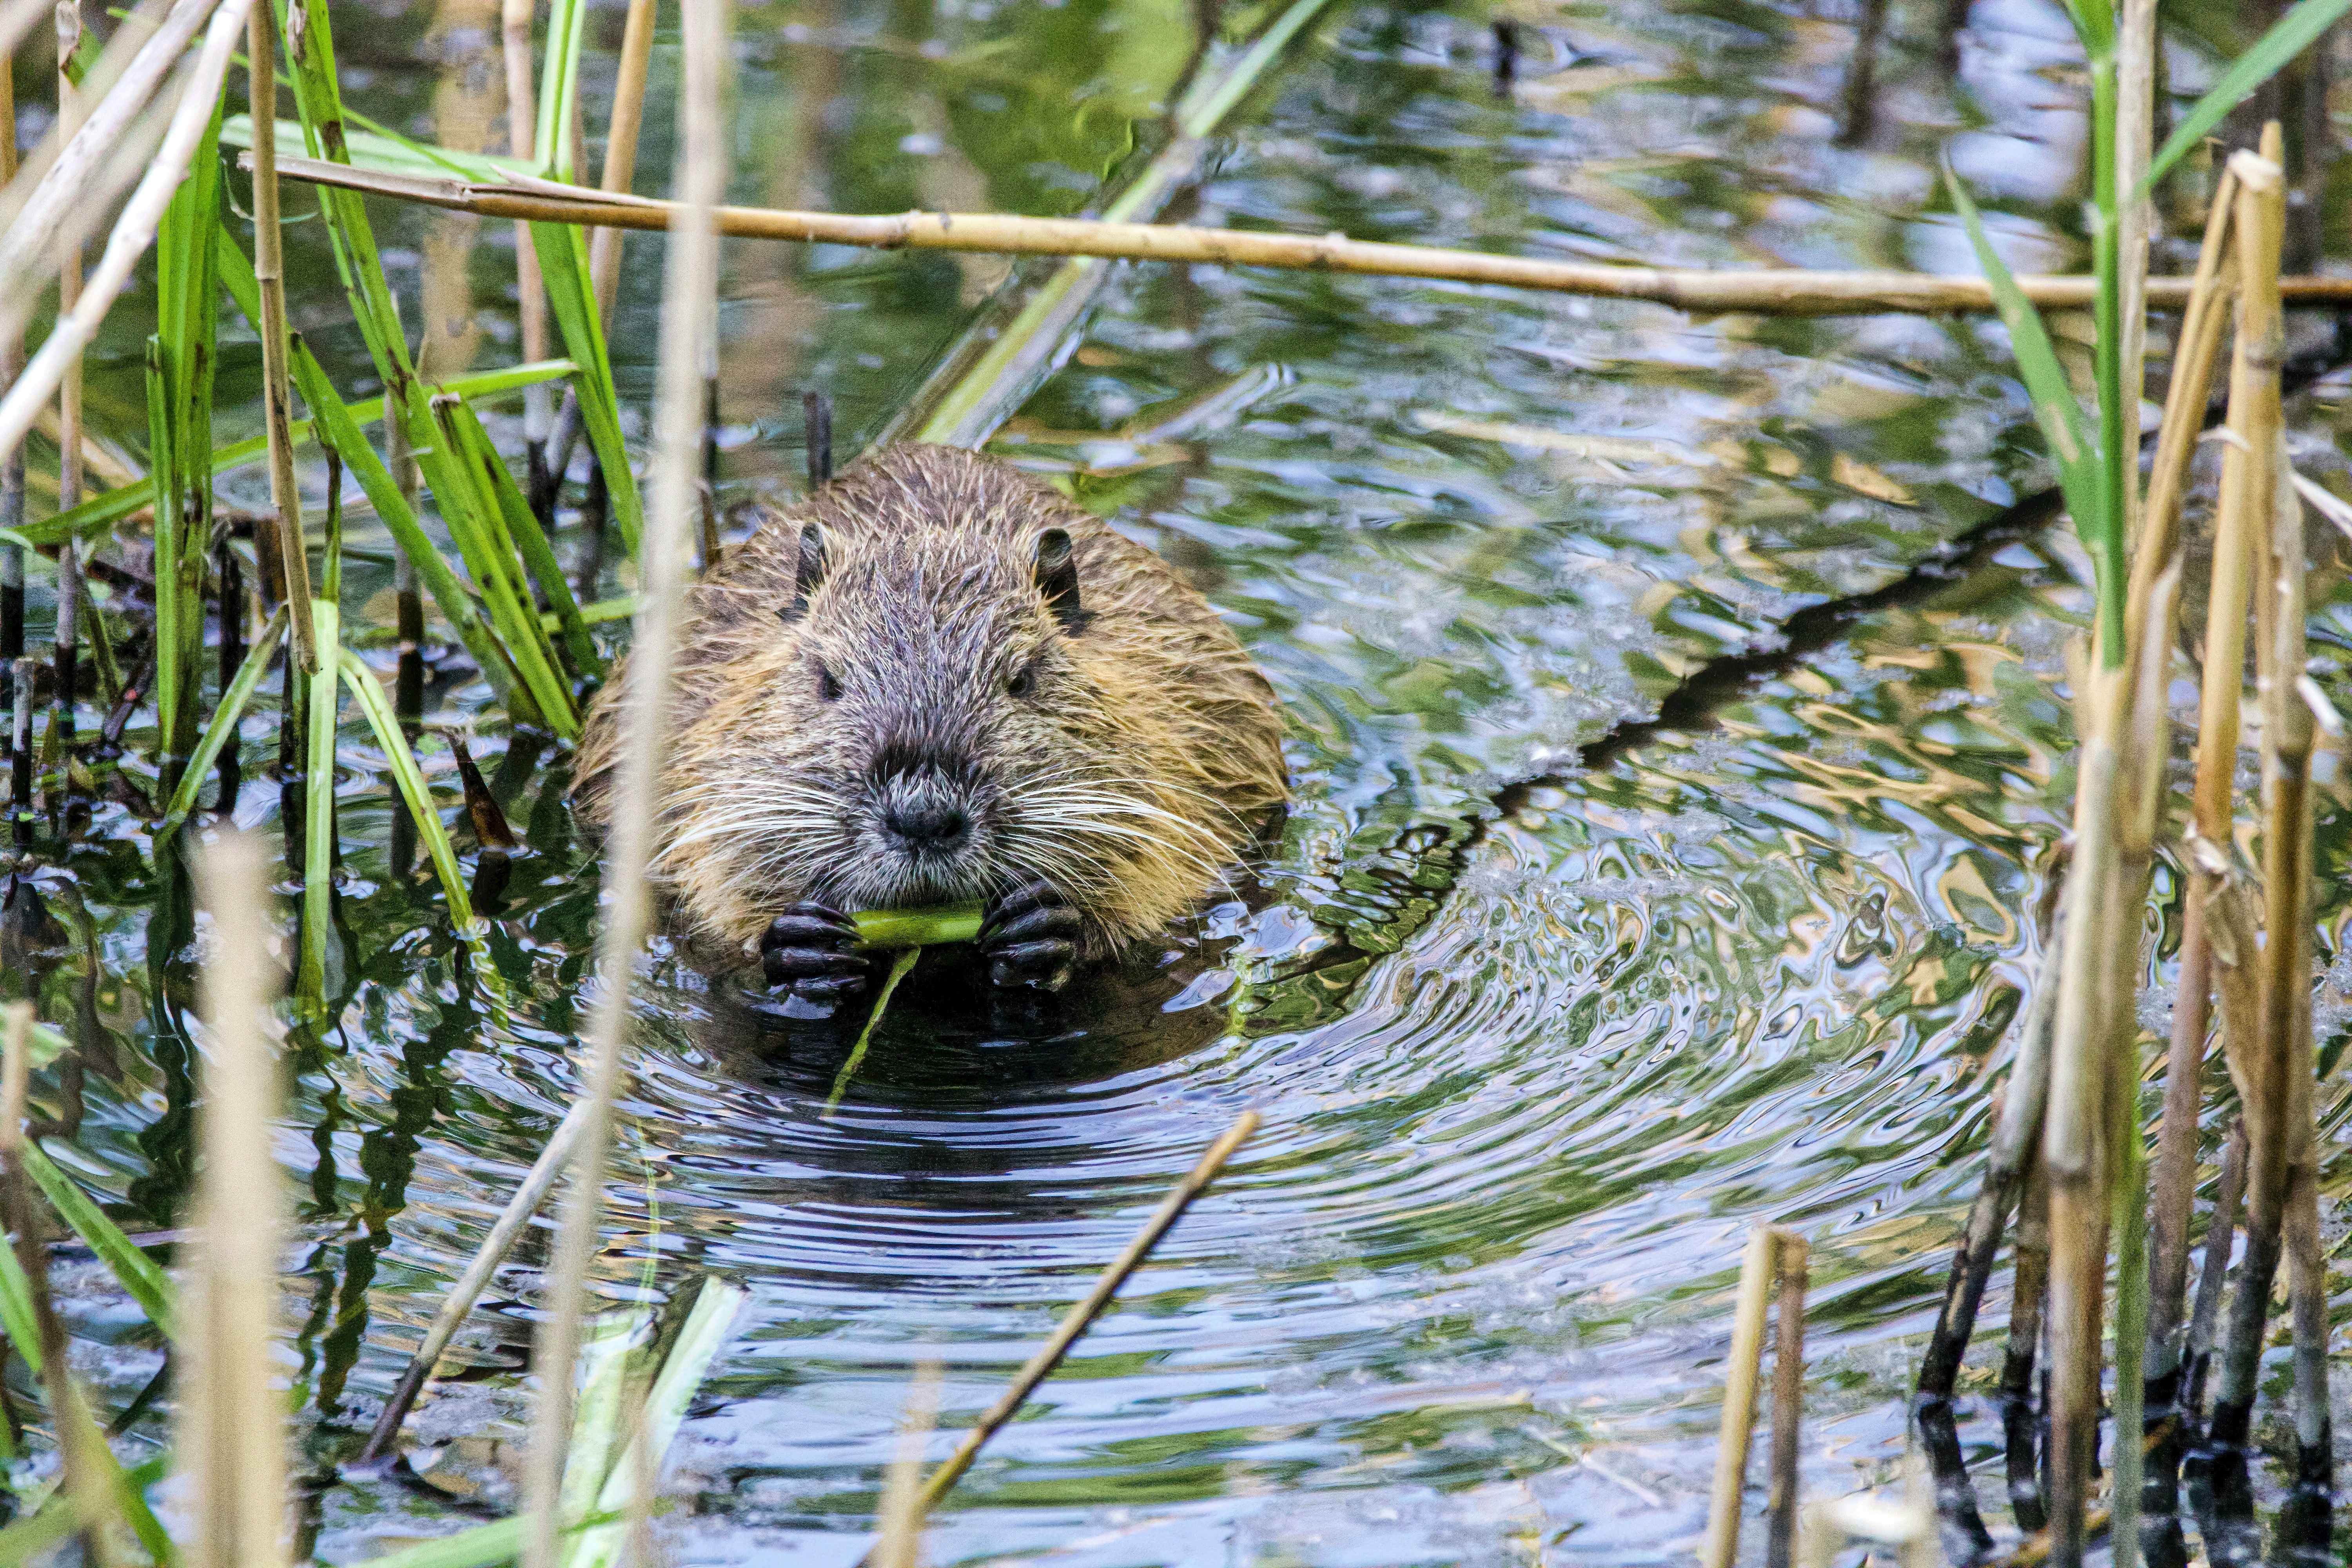
\includegraphics[width=0.6\textwidth]{Billeder/beaver.jpg}
	\end{center}
	I 
\end{opgavetekst}
\begin{delopgave}{1}
	Anvend regression for at bestemme tallene $a$ og $b$
\end{delopgave}
\begin{delopgave}{2}
	Forklar, hvad tallene $a$ og $b$ betyder for omsætningen på is. 
\end{delopgave}
%
%
%
%
%
\begin{opgavetekst}{Opgave 10}
	Tre ligninger er givet ved
	\begin{align*}
		&2x + 5y + 3z = 1,\\
		&4x + 10y - 4z = 3,\\
		&6x - y + 15z = -4.
	\end{align*}
\end{opgavetekst}
\begin{delopgave}{1}
	Bestem løsningen til ligningssystemet. 
\end{delopgave}
%
%
%
%
%
\newpage
\begin{opgavetekst}{Opgave 11}
	\begin{center}
		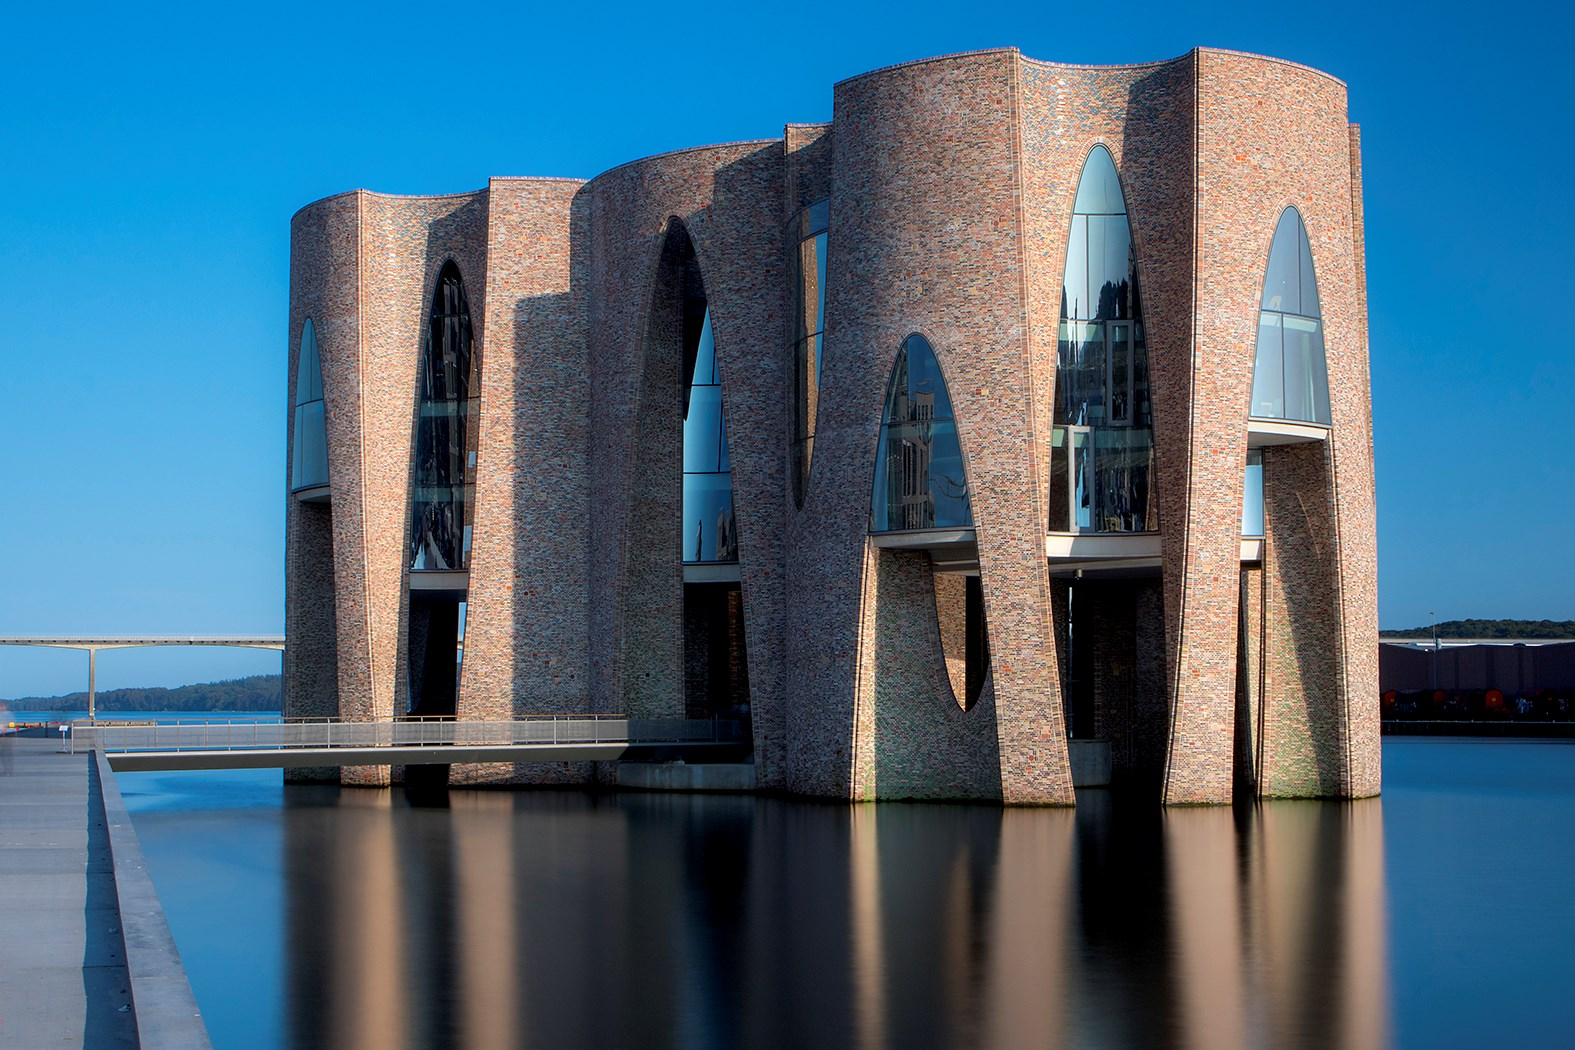
\includegraphics[width = 0.6\textwidth]{Billeder/Fjordenhus}
	\end{center}
	I Vejle ligger Fjordenhus, der som en del af facaden har parabellignende buer. Én af buerne kan ses indlejret i et koordinatsystem på Figur \ref{fig:fjordenhus}.
	\begin{figure}[H]
		\centering
		\begin{tikzpicture}
			\begin{axis}[
				axis lines = middle, 
				xmin = -2.5, 
				xmax = 20.5,
				ymin = -1.5,
				ymax = 22.5,
				xlabel = {$x$ (meter)},
				ylabel = {$y$ (meter)},
				xtick = {1.47,4,6.53},
				ytick = {12,20}
			]
				\addplot[color = teal, thick, samples = 150, domain = 0:8] {-1.25*x^2+10*x};
				\draw[color = teal, thick] (axis cs: 1.47,12) -- (axis cs: 6.53,12);
				\draw[color = teal, thick] (axis cs: 2.41,16.84) -- (axis cs: 5.59,16.84);
				\draw[color = teal, thick] (axis cs: 3.6,19.8) -- (axis cs: 3.6,16.84);
				\draw[color = teal, thick] (axis cs: 4.4,16.84) -- (axis cs: 4.4,12);
				\filldraw[color = olive] (axis cs: 1.47,12) circle (2pt);
				\filldraw[color = olive] (axis cs: 6.53,12) circle (2pt);
				\filldraw[color = olive] (axis cs: 4,20) circle (2pt);
				\draw[color = olive, dashed] (axis cs: 1.47,0) -- (axis cs: 1.47,12);
				\draw[color = olive, dashed] (axis cs: 1.47,12) -- (axis cs: 0,12);
				\draw[color = olive, dashed] (axis cs: 6.53,12) -- (axis cs: 0,12);
				\draw[color = olive, dashed] (axis cs: 6.53,12) -- (axis cs: 6.53,0);
				\draw[color = olive, dashed] (axis cs: 4,0) -- (axis cs: 4,20);
				\draw[color = olive, dashed] (axis cs: 4,20) -- (axis cs: 0,20);
			\end{axis}
		\end{tikzpicture}
		\caption{Skitse af facadeparabel på Fjordenhus.}
		\label{fig:fjordenhus}
	\end{figure}
	\phantom{h}
\end{opgavetekst}
\begin{delopgave}{1}
	Bestem en forskrift for den parabel, der fremgår af Figur \ref{fig:fjordenhus}.
\end{delopgave}
\begin{delopgave}{2}
	Afgør, hvor bred facadebuen på Fjordenhus er i vandoverfladen. 
\end{delopgave}
%
%
%
%
%

\phantom{h}
\newpage
\begin{center}
	\LARGE Bilag:
\end{center}
\begin{table}[H]
	\centering
	\begin{tikzpicture}
	\node at (0,0) {$v$};
	\node at (2*0.9,0) {$\cos(v)$};
	\node at (4*0.9,0) {$\sin(v)$};
	\node at (6*0.9,0) {$\tan(v)$};
	\node at (8*0.9,0) {$v$};
	\node at (10*0.9,0) {$\cos(v)$};
	\node at (12*0.9,0) {$\sin(v)$};
	\node at (14*0.9,0) {$\tan(v)$};
	\scriptsize
	%Colors
	\foreach \i in {0,...,22}{
		\filldraw[color = teal!60, opacity = 0.4] (-0.9,-0.5-0.3+0.15-\i*0.3*2) rectangle
		 (14*0.9 + 0.9,-0.5-0.3-0.15-\i*0.3*2);
	}
	\foreach \i in {0,...,45}{
		%Macros for evaluating
		\pgfmathsetmacro{\cval}{cos(\i)}
		\pgfmathsetmacro{\sval}{sin(\i)}
		\pgfmathsetmacro{\tval}{tan(\i)}
		%First columns of values
		\node at (0,-0.5-\i*0.3) {$\i^{\circ}$};
		\node at (2*0.9,-0.5-\i*0.3) { \cval };
		\node at (4*0.9,-0.5-\i*0.3) { \sval };
		\node at (6*0.9,-0.5-\i*0.3) { \tval };
	}
	\foreach \i in {46,...,89}{
		%Macros
		\pgfmathsetmacro{\cval}{cos(\i)}
		\pgfmathsetmacro{\sval}{sin(\i)}
		\pgfmathsetmacro{\tval}{tan(\i)}
		%Second column
		\node at (8*0.9,-0.5-\i*0.3 + 46*0.3) {$\i^{\circ}$};
		\node at (10*0.9,-0.5-\i*0.3 + 46*0.3) { \cval };
		\node at (12*0.9,-0.5-\i*0.3 + 46*0.3) { \sval };
		\node at (14*0.9,-0.5-\i*0.3 + 46*0.3) { \tval };
	}
		\pgfmathsetmacro{\cval}{cos(90)}
		\pgfmathsetmacro{\sval}{sin(90)}
		\node at (8*0.9,-0.5-90*0.3 + 46*0.3) {$90^{\circ}$};
		\node at (10*0.9,-0.5-90*0.3 + 46*0.3) { \cval };
		\node at (12*0.9,-0.5-90*0.3 + 46*0.3) { \sval };
	\end{tikzpicture}
	\caption{Tabel over udvalgte værdier for $\cos$, $\sin$ og $\tan$.}
	\label{tab:cossintan}
\end{table}
\end{document}




